% !TEX root = ../../main.tex
\section{Overview}\label{sec:method_overview}

\begin{figure}
  \centering
    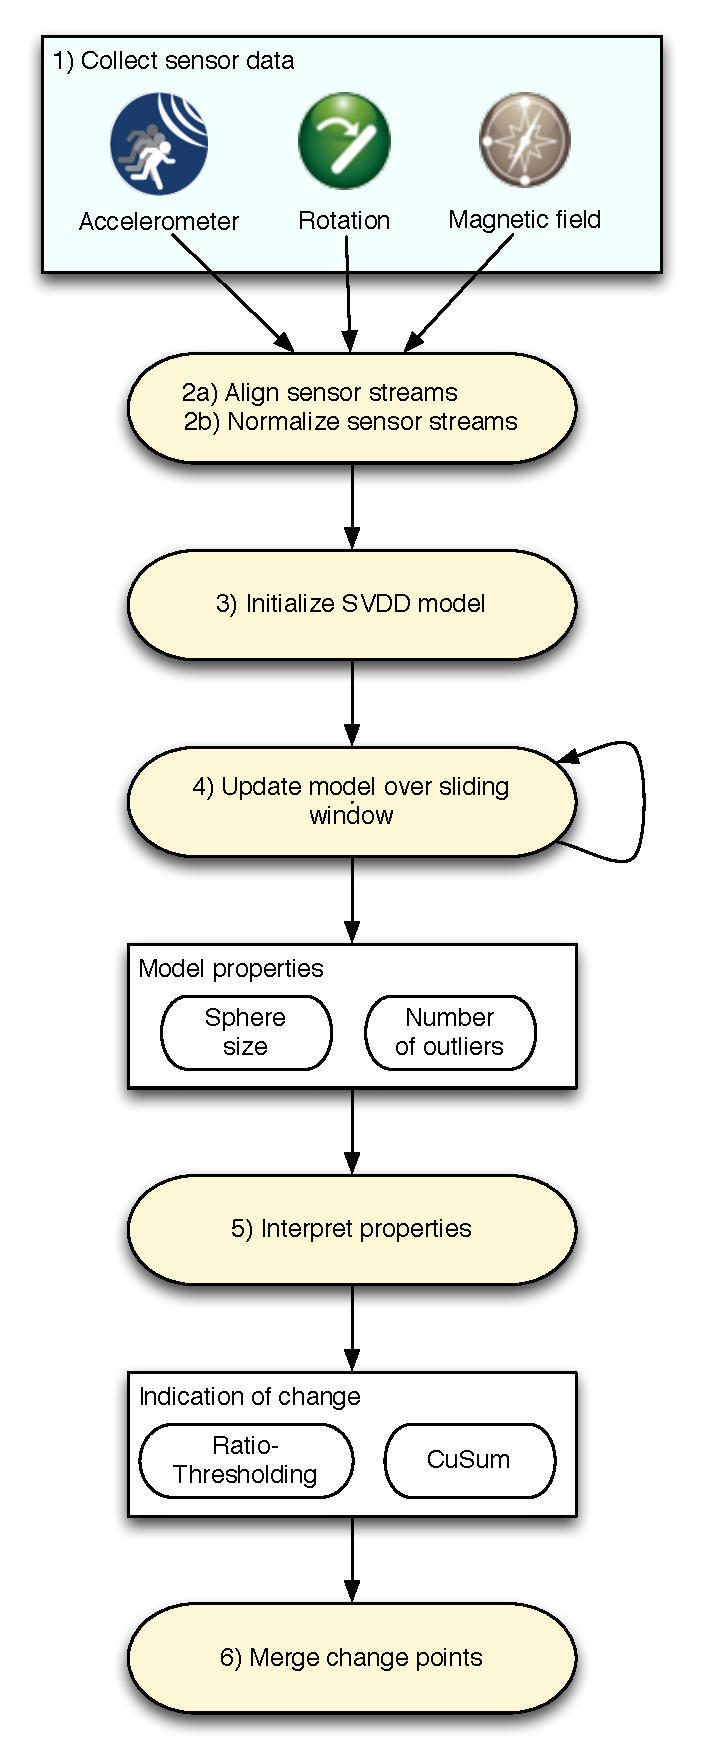
\includegraphics{./Figures/graphs/chapter4/method_setup.pdf}
  \caption[Method setup]{Schematic representation of the change detection method.}
  \label{fig:method_overview}
\end{figure}

This section gives a description of the method used for the experiments and change detection mechanism.
First described is the method to process the gathered sensor data.
A schematic overview is given in figure \ref{fig:method_overview} and shows the steps of the method.
A more detailed explanation of the ``Update model'' step follows.
This section is finalized with the experiments setup, annotation of data streams and quality measure.

\subsection{Change detection method}
As graphically represented in figure \ref{fig:method_overview}, the change detection method starts by processing the data from sensor, such as the accelerometer, magnetic orientation and rotation meaures \footnote{Something about the origin of the streams; all from the same sensor or different sensors?}.

The first step is to process the raw streams of data originating from a multiple of sensors.
The two processes applied are alignment and normalization.
Due to noisy sampling, not all the timestamps in the data streams are sensored at the same timestamp.
Since the \gls{svdd} method requires all the data stream at every timestamp and can not handle missing data on one of the timestamps, all the unique timestamps are filtered out.
Whilst this results in an overall filtering effect, in practice between $1\%$ and $5\%$ of each data stream is disregarded.
The effect of this filtering is not significant and the data is not modified.

Due to the nature of the sensor signals, a normalization step is required in order to set the weight for all the data streams equal.
The range of the accelerometer signal typically spans $-20$ to $20$, the magnetic field from $-45$ to $45$ and the rotations range is from $-1$ to $1$.
This means that a relative small change in the accelerometer stream could have a much larger impact on the model than the same (absolute) change in the rotation stream, whilst the latter has a larger relative impact.
The normalization step ensures that all data is weighted equally and changes in the data are all proportional.

In step $3$ the \gls{svdd} model is initialized.
The first full window over the data stream is used to construct an initial model.
During the initialization the parameters for the \gls{svdd} are provided, begin the kernel type (radial), \gls{rbf} with $\sigma$ and the outlier-fraction $C$.

Step $4$ is executed for every step-size $s$ data points in the stream.
Every update the oldest $s$ data points are removed from and $s$ new data points are added to the \gls{svdd} model.


\subsection{Model updating}

\subsection{Experiments}